\documentclass[twocolumn]{article}

\usepackage{preprint}
\usepackage{graphicx}
\usepackage{tikz}
\usepackage{adjustbox}
\usepackage[most]{tcolorbox}
\usepackage{xcolor}
\usepackage{wrapfig}
\usepackage[hidelinks]{hyperref}

\title{Reproducible experiments using OpenTTD}
\author{Michal Charemza}
\date{April 2023}

% Based on https://www.overleaf.com/latex/templates/sticky-notes/ftrvjddrmbwx
% Vebjørn S. Førde
% Creative Commons CC BY 4.0
% Yellow:
\definecolor{BgYellow}{HTML}{FFF59C}
\definecolor{FrameYellow}{HTML}{F7A600}
\newtcolorbox{YStkyNote}[1][]{%
    enhanced,
    before skip=2mm,after skip=2mm, 
    width=\columnwidth - 3mm, % width of the sticky note
    boxrule=0.2mm,
    colback=BgYellow, colframe=FrameYellow, % Colors
    attach boxed title to top left={xshift=0cm,yshift*=0mm-\tcboxedtitleheight},
    varwidth boxed title*=-3cm,
    % The titlebox:
    boxed title style={frame code={%
        \path[left color=FrameYellow,right color=FrameYellow,
        middle color=FrameYellow]
        ([xshift=-0mm]frame.north west) -- ([xshift=0mm]frame.north east)
        [rounded corners=0mm]-- ([xshift=0mm,yshift=0mm]frame.north east)
        -- (frame.south east) -- (frame.south west)
        -- ([xshift=0mm,yshift=0mm]frame.north west)
        [sharp corners]-- cycle;
        },interior engine=empty,
    },
    sharp corners,rounded corners=southeast,arc is angular,arc=3mm,
    % The "folded paper" in the bottom right corner:
    underlay={%
        \path[fill=BgYellow!80!black] ([yshift=3mm]interior.south east)--++(-0.4,-0.1)--++(0.1,-0.2);
        \path[draw=FrameYellow,shorten <=-0.05mm,shorten >=-0.05mm,color=FrameYellow] ([yshift=3mm]interior.south east)--++(-0.4,-0.1)--++(0.1,-0.2);
        },
    drop fuzzy shadow, % Shadow
    fonttitle=\bfseries, 
    title={#1}
}

\begin{document}

\twocolumn[
  \begin{@twocolumnfalse}
  
    \maketitle

    \begin{abstract}
        OpenTTD is an open source real time strategy (RTS) business simulation game based on the 1994 game Transport Tycoon Deluxe. In spite of being designed as a recreational game, OpenTTD has been the focus of a number of academic studies. However, these studies have problems regarding the reproducibility of their experiments. This paper summarises the problems, and suggests extensions to OpenTTD to avoid these problems in future.
    \end{abstract}
\vspace{0.35cm}

  \end{@twocolumnfalse}
]

\section{Introduction}

OpenTTD \cite{openttd} is an open source real time strategy (RTS) simulation game. The aim of the game is to successfully run a business by constructing networks of roads, railways, airports and ports, along with their respective vehicles, trains, planes and ships, in order to transport people and goods in exchange for money. OpenTTD is played on two dimensional isometric grid as can be seen in Figure \ref{fig:openttd}.

\begin{figure}[h]
\centering
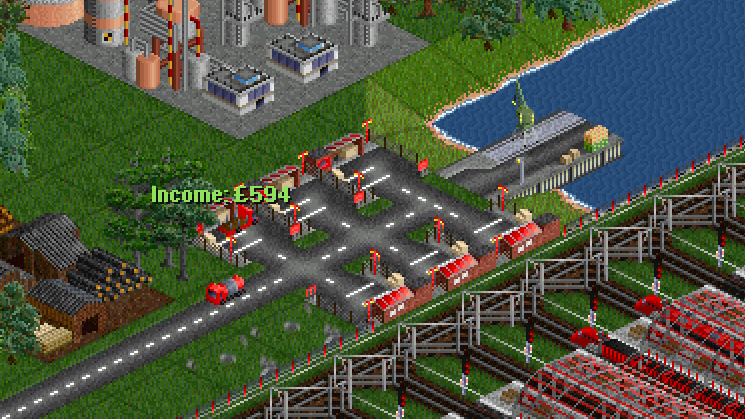
\includegraphics[width=\columnwidth]{assets/openttd-screenshot.png}
\caption{A small section of an OpenTTD (version 12.2) game at the moment when income is received for delivering goods by road. Also shown is part of a railway network, a port for ships, an oil refinery, and a sawmill.}
\label{fig:openttd}
\end{figure}

OpenTTD has been designed as a game for recreation. However, it is remarkably flexible: it has been successfully used as a tool to research algorithms, scalability, mobile applications, and as a teaching aid \cite{HansenMuprhie2018}. Using it a a tool for research is the focus of this paper, and specifically its features for reproducible research.

\section{Reproducibility, Replicatability, \& Repeatability}
\begin{YStkyNote}[TODO]
Explain the differences
\end{YStkyNote}

\section{Review of research using OpenTTD}

\begin{YStkyNote}[TODO]
Give specific examples of the issues in research
\end{YStkyNote}

\section{Review of OpenTTD configuration}

\begin{YStkyNote}[TODO]
Explain some of the configuration that is useful for reproducibility
\end{YStkyNote}

\section{Possible extensions to OpenTTD}

\begin{YStkyNote}[TODO]
Suggest extensions that would address the issues of the research
\end{YStkyNote}

\section{Research vs. recreation}

\begin{YStkyNote}[TODO]
OpenTTD is a game, and not for research. Is there a tension? Could it be for both?
\end{YStkyNote}

\section{Conclusion}

\begin{YStkyNote}[TODO]
Briefly repeat the main points above
\end{YStkyNote}

\normalsize
\bibliographystyle{unsrt}
\bibliography{main}

\end{document}
